\section{Wielkość zatrudnienia, schemat struktury organizacyjnej}

\begin{table}[h]
	\centering
	\caption{Wielkość zatrudnienia -- schemat struktury zatrudnienia}
	\begin{tabular}{*{4}{p{0.2\textwidth}}}
		\hline
		\multirow{2}{*}{Dział} & \multirow{2}{*}{Stanowisko} & \multicolumn{2}{l}{\makecell[l]{Godziny pracy i \\ liczba pracowników}} \\
		\cline{3-4}
		& & Zmiana 1 & Zmiana 2 \\
		\hline\hline
		\multirow{4}{*}{Zarząd}& Dyrektor Naczelny & 8:00 - 16:00 (1 osoba) \\
		\cline{2-4}
		 & Dyrektor ds. Sprzedaży i Marketingu & 8:00 - 16:00 (1 osoba) \\
		\cline{2-4}
		 & Dyrektor ds. Produkcji & 7:00 - 15:00 (1 osoba) \\
		\cline{2-4}
		 & Dyrektor ds. Ekonomiczno - Finansowych & 8:00 - 16:00 (1 osoba) \\
		 \hline
		\multirow{8}{*}{Administracja} & Pełnomocnik ds. Systemu Zarządzania & 9:00 - 17:00 (1 osoba) \\
		\cline{2-4}
		 & Kierownik Administracji & 6:00 - 14:00 (1 osoba) \\
		\cline{2-4}
		 & Zastępca Kierownika Administracji & 14:00 - 20:00 (1 osoba) \\
		\cline{2-4}
		 & Księgowość & 6:00 - 14:00 (2 osoby) & \\
		\cline{2-4}
		 & Sekretariat & 8:00 - 16:00 (1 osoba) \\
		\cline{2-4}
		 & Pracownik ochrony & 6:00 - 14:00 (1 osoba) & 14:00- 22:00 ( 1 osoba) / 22:00 - 6:00 (1 osoba) \\
		\cline{2-4}
		 & Personel sprzątający & 6:00 - 14:00 (3 osoby) & 14:00 - 22:00 (3 osoby) \\
		\cline{2-4}
		 & Kierowca & 6:00 - 14:00 (1 osoba) & 14:00 - 22:00 (1 osoby) \\
		 \hline
		Ekonomiczno - Finansowy & Specjalista ds. Kadr i Płac & 8:00 - 16:00 (2 osoby) \\
		\hline
		Organizacja, Zarządzanie i Kontrola Jakością & Specjalista ds. Organizacji, Zarządzania i Kontroli Jakości & 6:00 - 14:00 (1 osoba) & 14:00 - 22:00 (1 osoba) \\
		\hline
		Sprzedaży i Marketingu & Specjalista ds. Sprzedaży i Marketingu & 8:00 - 16:00 (2 osoby) \\
		\hline
		Informatyki & Informatyk & 9:00 - 17:00 (1 osoba) \\
		\hline
		\multirow{4}{*}{Produkcja} & Kierownik Produkcji & 6:00 - 14:00 (1 osoba) & 14:00 - 22:00 (1 osoba) \\
		\cline{2-4}
		 & Pracownik odpowiedzialny za odbiór i składowanie towaru & 6:00 - 14:00 (3 osoby) & 14:00 - 22:00 (3 osoby) \\
		\cline{2-4}
		 & Prcownik odpowiedzialny za proces produkcji i obsługi maszyn & 6:00 - 14:00 (10 osób) & 14:00 - 22:00 (10 osób) \\
		\cline{2-4}
		 & Pracownik odpowiedzialny za proces pakowania & 6:00 - 14:00 (5 osób) & 14:00 - 22:00 (5 osób) \\
		 \hline
	\end{tabular}
\end{table}

W zakładzie zatrudnionych jest łącznie 68 osób. W zakładzie obowiązuje produkcja w godzinach 6:00 – 22:00, z tego powodu w harmonogramie czasu pracy ustalone zostały 2 zmiany w godzinach 6:00 – 14:00 oraz 14:00 – 22:00. Osoby zatrudnione rozdzielone zostały na 8 działów:
\begin{itemize}
	\item \textsf{Zarząd},
	\item \textsf{Administracja},
	\item \textsf{Dział Ekonomiczno – Finansowy},
	\item\textsf{Dział Organizacji, Zarządzania i Kontroli Jakości},
	\item\textsf{Dział Sprzedaż i Marketingu},
	\item \textsf{Dział Informatyki}
	\item \textsf{Dział Produkcji}. 
\end{itemize}

\begin{figure}[H]
	\centering
	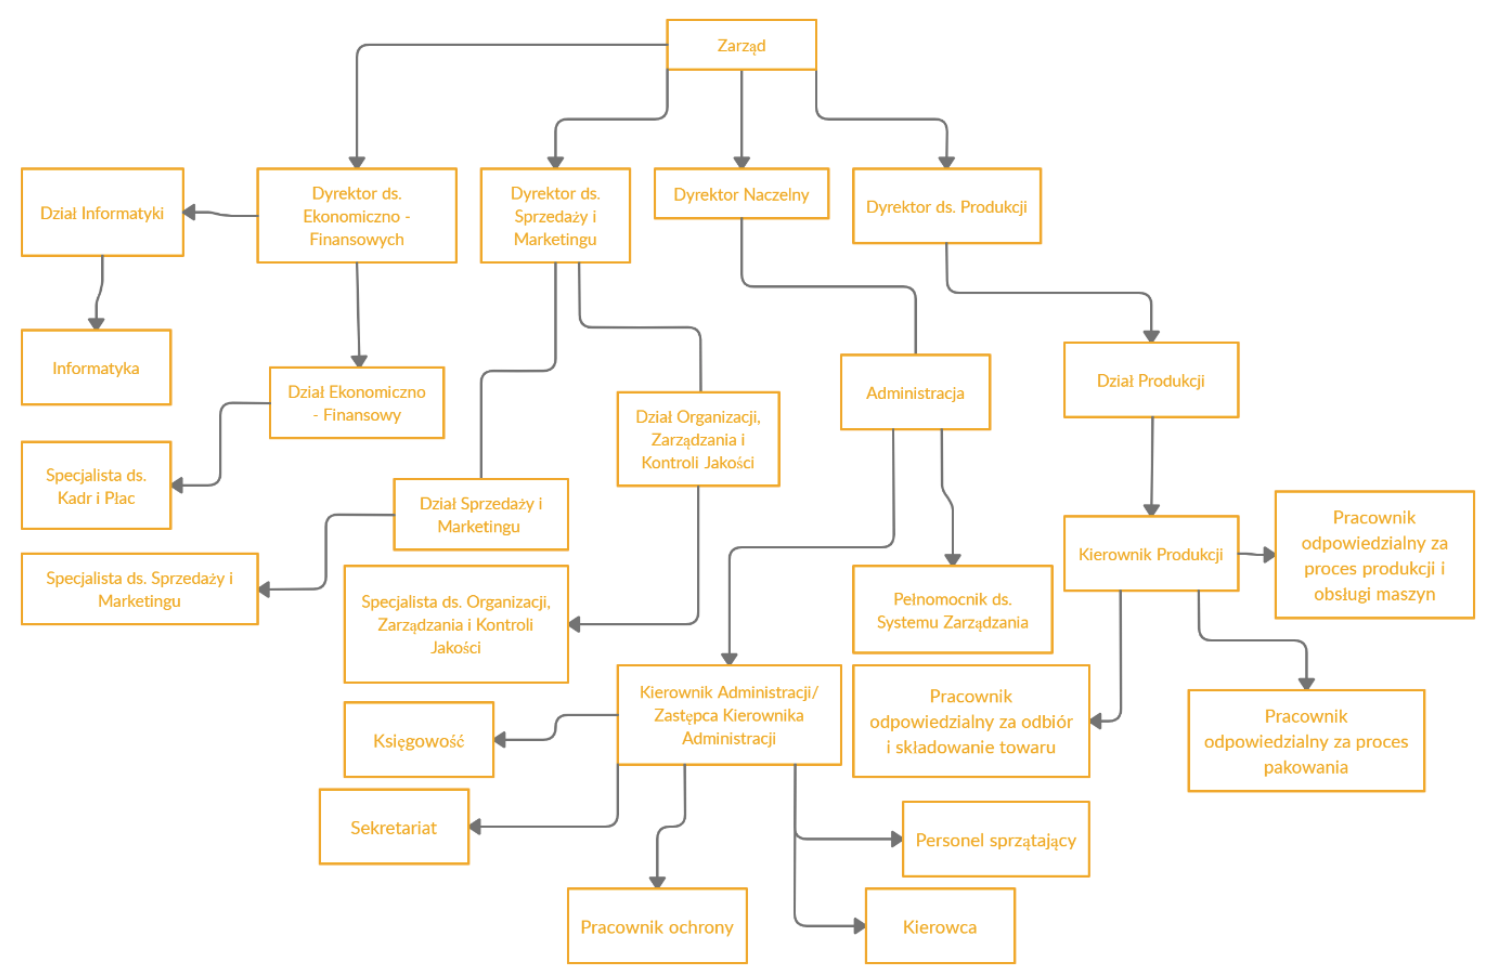
\includegraphics[width=0.8\textwidth]{./sec17/struktura_organizacyjna.png}
	\caption{Schemat struktury organizacyjnej (autor: Grzegorz Jakubiak)}
\end{figure}

		Została wybrana taka liczba pracowników, gdyż według kodeksu pracy musi być zachowana doba pracownicza, co oznacza, że wymagane jest 11h odpoczynku, a czas pracy nie może przekraczać 8h na dobę oraz 48h tygodniowo w przyjętym okresie rozliczeniowym. 
